% ------------------------------------------------------------------------------
% TYPO3 Version 10.3 - What's New (Dutch Version)
%
% @license	Creative Commons BY-NC-SA 3.0
% @link		https://typo3.org/help/documentation/whats-new/
% @language	Dutch
% ------------------------------------------------------------------------------

\section{Wijzigingen voor ontwikkelaars}
\begin{frame}[fragile]
	\frametitle{Wijzigingen voor ontwikkelaars}

	\begin{center}\huge{Hoofdstuk 3:}\end{center}
	\begin{center}\huge{\color{typo3darkgrey}\textbf{Wijzigingen voor ontwikkelaars}}\end{center}

\end{frame}

% ------------------------------------------------------------------------------
% Feature | 90333 | Dashboard

\begin{frame}[fragile]
	\frametitle{Wijzigingen voor ontwikkelaars}
	\framesubtitle{Dashboard (1)}

	% decrease font size for code listing
	\lstset{basicstyle=\smaller\ttfamily}

	\begin{itemize}
		\item Ontwikkelaars kunnen maatwerk widgets voor het Dashboard maken door een van de volgende widget \textit{abstracts} uit te breiden:

			\begin{itemize}
				\item \texttt{AbstractWidget}\newline
					\small
						Een basis-abstract die kan worden gebruikt als basis voor eenvoudige widgets.
					\normalsize
				\item \texttt{AbstractRssWidget}\newline
					\small
						Een abstract om een widget te maken die een RSS-feed toont.
					\normalsize
				\item \texttt{AbstractListWidget}\newline
					\small
						Een abstract om een widget te maken die een lijst toont.
					\normalsize
				\item \texttt{AbstractCtaButtonWidget}\newline
					\small
						Een abstract voor een widget die een "actie"-knop toont.
					\normalsize
			\end{itemize}

	\end{itemize}

\end{frame}

% ------------------------------------------------------------------------------
% Feature | 90333 | Dashboard

\begin{frame}[fragile]
	\frametitle{Wijzigingen voor ontwikkelaars}
	\framesubtitle{Dashboard (2)}

	% decrease font size for code listing
	\lstset{basicstyle=\tiny\ttfamily}

	\begin{itemize}
		\item Eigen widgets worden in het volgende bestand in een extensie geregistreerd:\newline
			\texttt{EXT:my\_extension/Configuration/Services.yaml}

		\item Optie 1: widget-identifier als attribuut

\vspace{-0.4cm}
\begin{lstlisting}
Vendor\MyExtension\Widgets\MyFirstWidget:
  tags:
    - name: dashboard.widget
      identifier: widget-identifier-1
      widgetGroups: 'general'
\end{lstlisting}

		\item Optie 2: eigen servicenaam laat meerdere widget-identifier een klasse delen

\vspace{-0.4cm}
\begin{lstlisting}
widget.identifier:
  class: Vendor\MyExtension\Widgets\MySecondWidget
  tags:
    - name: dashboard.widget
      identifier: widget-identifier-2
      widgetGroups: 'general, typo3'
\end{lstlisting}

	\end{itemize}

\end{frame}

% ------------------------------------------------------------------------------
% Feature | 90333 | Dashboard

\begin{frame}[fragile]
	\frametitle{Wijzigingen voor ontwikkelaars}
	\framesubtitle{Dashboard (3)}

	% decrease font size for code listing
	\lstset{basicstyle=\tiny\ttfamily}

	\begin{itemize}
		\item Elke widget is gekoppeld aan een of meer widgetgroepen.
		\item Deze groepen staan in de popup bij het toevoegen van een nieuwe widget aan een dashboard.
		\item Ontwikkelaars kunnen eigen widgetgroepen configureren door een bestand aan te maken\newline
			\smaller
				\texttt{EXT:my\_extension/Configuration/Backend/DashboardWidgetGroups.php}
			\normalsize

\vspace{-0.4cm}
\begin{lstlisting}
return [
  'widgetGroup-exampleGroup' => [
    'title' => 'LLL:EXT:my_extension/Resources/Private/Language/locallang.xlf:widget_group_name',
  ],
];
\end{lstlisting}

	\end{itemize}

\end{frame}

% ------------------------------------------------------------------------------
% Feature | 89870 | New PSR-14 Events for Extbase-related signals

\begin{frame}[fragile]
	\frametitle{Wijzigingen voor ontwikkelaars}
	\framesubtitle{Extbase en Fluid}

	% decrease font size for code listing
	\lstset{basicstyle=\tiny\ttfamily}

	\begin{itemize}
		\item De volgende PSR-14-gebaseerde events zijn toegevoegd aan signals in Extbase:

\vspace{-0.4cm}
\begin{lstlisting}
TYPO3\CMS\Extbase\Event\Mvc\AfterRequestDispatchedEvent
TYPO3\CMS\Extbase\Event\Mvc\BeforeActionCallEvent
TYPO3\CMS\Extbase\Event\Persistence\AfterObjectThawedEvent
TYPO3\CMS\Extbase\Event\Persistence\ModifyQueryBeforeFetchingObjectDataEvent
TYPO3\CMS\Extbase\Event\Persistence\ModifyResultAfterFetchingObjectDataEvent
TYPO3\CMS\Extbase\Event\Persistence\EntityAddedToPersistenceEvent
TYPO3\CMS\Extbase\Event\Persistence\EntityFinalizedAfterPersistenceEvent
TYPO3\CMS\Extbase\Event\Persistence\EntityUpdatedInPersistenceEvent
TYPO3\CMS\Extbase\Event\Persistence\EntityRemovedFromPersistenceEvent
TYPO3\CMS\Extbase\Event\Persistence\EntityPersistedEvent
\end{lstlisting}

		\item Bestaande signals zijn vervangen en moeten niet meer gebruikt worden.

	\end{itemize}

\end{frame}

% ------------------------------------------------------------------------------
% Feature | 89644 | Add optional argument fields to editRecord ViewHelpers

\begin{frame}[fragile]
	\frametitle{Wijzigingen voor ontwikkelaars}
	\framesubtitle{ViewHelper \texttt{editRecord}}

	% decrease font size for code listing
	\lstset{basicstyle=\tiny\ttfamily}

	\begin{itemize}
		\item De \texttt{uri.editRecord} en \texttt{link.editRecord} ViewHelpers hebben een
			optioneel argument \texttt{fields} gekregen.
		\item Indien aanwezig maakt de FormEngine een formulier om alleen de opgegeven databasevelden te bewerken.
		\item Het volgende voorbeeld maakt een link om het veld \texttt{tt\_content.bodytext}
			te bewerken van het record met UID 42.

\begin{lstlisting}
<be:link.editRecord uid="42" table="tt_content" fields="bodytext" returnUrl="foo/bar">
  Edit record
</be:link.editRecord>
\end{lstlisting}

	\end{itemize}

\end{frame}

% ------------------------------------------------------------------------------
% Feature | xxxxx | Introduce AssetCollector

\begin{frame}[fragile]
	\frametitle{Wijzigingen voor ontwikkelaars}
	\framesubtitle{AssetCollector}

	\begin{itemize}
		\item De eerste stappen voor het integreren van een AssetCollector zijn gereed.
		\item Het concept maakt het mogelijk om eigen CSS/JS (inline of extern) meerdere
			keren toe te voegen maar slecht één keer uit te voeren.
		\item Hiervoor zijn twee nieuwe Fluid ViewHelpers toegevoegd:
			\begin{itemize}
				\item \texttt{<f:css>}
				\item \texttt{<f:script>}
			\end{itemize}
		\item Op lange termijn zal de AssetCollector de verschillende TypoScript opties
			die nogal verwarrend zijn vervangen.
	\end{itemize}

\end{frame}

% ------------------------------------------------------------------------------
% Feature | 86614 | Add PSR-14 event to control hreflang tags to be rendered

\begin{frame}[fragile]
	\frametitle{Wijzigingen voor ontwikkelaars}
	\framesubtitle{Wijzig \texttt{hreflang}-tag}

	% decrease font size for code listing
	\lstset{basicstyle=\smaller\ttfamily}

	\begin{itemize}
		\item De \texttt{hreflang} tags kunnen gewijzigd worden voordat ze uitgevoerd worden.
		\item Ontwikkelaars kunnen dit bereiken door het registreren van een event listener voor dit event:\newline
			\smaller
				\texttt{TYPO3\textbackslash
					CMS\textbackslash
					Frontend\textbackslash
					Event\textbackslash
					ModifyHrefLangTagsEvent}
			\normalsize
	\end{itemize}

\end{frame}

% ------------------------------------------------------------------------------
% Feature | 88818 | Introduce events to modify CKEditor configuration

\begin{frame}[fragile]
	\frametitle{Wijzigingen voor ontwikkelaars}
	\framesubtitle{CKEditor configuratie wijzigen}

	% decrease font size for code listing
	\lstset{basicstyle=\tiny\ttfamily}

	\begin{itemize}
		\item Met de volgende PSR-14-gebaseerde events kan de CKEditorconfiguratie worden gewijzigd:

\vspace{-0.4cm}
\begin{lstlisting}
TYPO3\CMS\RteCKEditor\Form\Element\Event\AfterGetExternalPluginsEvent
TYPO3\CMS\RteCKEditor\Form\Element\Event\BeforeGetExternalPluginsEvent
TYPO3\CMS\RteCKEditor\Form\Element\Event\AfterPrepareConfigurationForEditorEvent
TYPO3\CMS\RteCKEditor\Form\Element\Event\BeforePrepareConfigurationForEditorEvent
\end{lstlisting}

		\item De
			\href{https://docs.typo3.org/c/typo3/cms-core/master/en-us/Changelog/10.3/Feature-88818-IntroduceEventsToModifyCKEditorConfiguration.html}{lijst wijzigingen}
			bevat een voorbeeld.
	\end{itemize}

\end{frame}

% ------------------------------------------------------------------------------
% Feature | 90265 | Show dispatched Events in Admin Panel

\begin{frame}[fragile]
	\frametitle{Wijzigingen voor ontwikkelaars}
	\framesubtitle{PSR-14 Events in Admin Panel}

	\begin{itemize}
		\item Het Admin Panel toont alle PSR-14 events die in het huidige pagina zijn aangeroepen.
	\end{itemize}

	\begin{figure}
		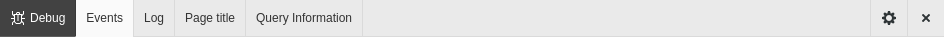
\includegraphics[width=0.85\linewidth]{ChangesForDevelopers/90265-ShowDispatchedEventsInAdminPanel.png}
	\end{figure}

\end{frame}

% ------------------------------------------------------------------------------
% Feature | 89738 | API for AJAX Requests

\begin{frame}[fragile]
	\frametitle{Wijzigingen voor ontwikkelaars}
	\framesubtitle{API voor AJAX Requests}

	% decrease font size for code listing
	\lstset{basicstyle=\tiny\ttfamily}

	\begin{itemize}
		\item De \textbf{Fetch API} is toegevoegd voor het maken van AJAX requests
			en om TYPO3 minder afhankelijk van jQuery te maken.
		\item De API biedt een generieke definitie van Request en Response objecten
			(en andere zaken omtrent een netwerkrequest)
		\item Ondersteund door alle moderne browsers, zie
			\href{https://developer.mozilla.org/en-US/docs/Web/API/Fetch_API}{compatibiliteitsoverzicht}.
		\item De TYPO3 core gebruikt de nieuwe API al in de Install Tool, FormEngine en
			contextmenu's.
		\item Zie de
			\href{https://docs.typo3.org/c/typo3/cms-core/master/en-us/Changelog/10.3/Feature-89738-ApiForAjaxRequests.html}{lijst wijzigingen}
			voor enkele voorbeelden voor het gebruik van de Fetch API.

	\end{itemize}

\end{frame}

% ------------------------------------------------------------------------------
% Feature | 89650 | Allow line breaks in TCA descriptions

\begin{frame}[fragile]
	\frametitle{Wijzigingen voor ontwikkelaars}
	\framesubtitle{TCA veld Beschrijving}

	\begin{itemize}
		\item Het veld Beschrijving in de TCA kan regeleindes bevatten om lange teksten beter leesbaar te maken.
	\end{itemize}

\end{frame}

% ------------------------------------------------------------------------------
% Important | 90020 | Legacy BasicFileUtility and ExtendedFileUtility classes marked as internal

\begin{frame}[fragile]
	\frametitle{Wijzigingen voor ontwikkelaars}
	\framesubtitle{Classes \texttt{BasicFileUtility} en \texttt{ExtendedFileUtility}}

	\begin{itemize}
		\item De volgende twee oude klassen zijn aangemerkt als \textbf{internal}
			en zouden niet meer gebruikt moeten worden:

			\begin{itemize}\small
				\item \texttt{TYPO3\textbackslash
					CMS\textbackslash
					Core\textbackslash
					Utility\textbackslash
					File\textbackslash
					BasicFileUtility}
				\item \texttt{TYPO3\textbackslash
					CMS\textbackslash
					Core\textbackslash
					Utility\textbackslash
					File\textbackslash
					ExtendedFileUtility}
			\end{itemize}

		\item Ontwikkelaars van extensies zouden de klasse \texttt{ResourceStorage}
			en \texttt{ResourceFactory} moeten gebruiken voor het beheer van assets.

	\end{itemize}

\end{frame}

% ------------------------------------------------------------------------------
% Feature | 89139 | Add dependency injection support for console commands

\begin{frame}[fragile]
	\frametitle{Wijzigingen voor ontwikkelaars}
	\framesubtitle{Console commando's: Symfony DI Ondersteuning}

	\begin{itemize}
		\item Afhankelijkheden kunnen nu geïnjecteerd worden via constructor of andere injectietechnieken.
		\item Voeg de \texttt{console.command} tag toe aan commando klassen.
		\item Gebruik het tag-attribuut \texttt{command} om de commandonaam te specificeren.
		\item De optionele tagattribuut \texttt{schedulable} kan ingesteld worden op \texttt{false}
			om het commando uit de Taakplanner te houden.

		\item Zie
			\href{https://docs.typo3.org/c/typo3/cms-core/master/en-us/Changelog/10.3/Feature-89139-AddDependencyInjectionSupportForConsoleCommands.html}{lijst wijzigingen}
			voor een voorbeeld.
	\end{itemize}

\end{frame}

% ------------------------------------------------------------------------------
% Feature | 90168 | Introduce Modal Actions

\begin{frame}[fragile]
	\frametitle{Wijzigingen voor ontwikkelaars}
	\framesubtitle{Actieknoppen in popups}

	% decrease font size for code listing
	\lstset{basicstyle=\tiny\ttfamily}

	\begin{itemize}
		\item Modal popups ondersteunen actieknoppen.
		\item Als een alternatief voor de bestaande \texttt{trigger}-optie kan de nieuwe
			optie \texttt{action} worden gebruikt.
		\item Bijvoorbeeld:

\vspace{-0.4cm}
\begin{lstlisting}
Modal.confirm('Header', 'Some content', Severity.error, [
  {
    text: 'Gebaseerd op trigger()',
    trigger: function () {
      console.log('Vintage!');
    }
  },
  {
    text: 'Gebaseerd op action()',
    action: new DeferredAction(() => {
      return new AjaxRequest('/any/endpoint').post({});
    })
  }
]);
\end{lstlisting}

	\end{itemize}

\end{frame}

% ------------------------------------------------------------------------------
% Feature | 90471 | JavaScript Event API

\begin{frame}[fragile]
	\frametitle{Wijzigingen voor ontwikkelaars}
	\framesubtitle{JavaScript Event API}

	\begin{itemize}
		\item Een nieuwe Event API geeft JavaScript ontwikkelaars een stabiel koppelvlak voor event listeners.
		\item De API handelt bekende valkuilen af zoals event delegation en event unbinding.
		\item Elke \textit{event strategy} biedt twee manieren om het te koppelen aan een listener
		\item De Event API biedt verschillende stategieën om even listeners af te handelen.
		\item Zie
			\href{https://docs.typo3.org/c/typo3/cms-core/master/en-us/Changelog/10.3/Feature-90471-JavaScriptEventAPI.html}{lijst wijzigingen}
			voor voorbeelden en verdere details.
	\end{itemize}

\end{frame}

% ------------------------------------------------------------------------------
